\chapter{Package Development} \label{cpt:Pkg Dev}

\section{Introduction}

In this chapter, we will elaborate on the development of \mintinline{R}|rmcop|. We will first present the general structure of the package. Then, we will discuss the implementation of pricing models mentioned in the literature review in Section \ref{sec:Literature Review} in details.

\section{Package Structure} \label{sec:Pkg Structure}

The overlying workflow of using \mintinline{R}|rmcop| package to price financial option is displayed in Figure \ref{img:flowchart_option} below. One shall see that with the OOP framework, we encapsulate most arguments into two classes of objects: \mintinline{R}|option| and \mintinline{R}|env|.

\begin{figure}[H]
    \centering
    % \def\svgwidth{\columnwidth}
    \includesvg[scale = 0.8]{flowchart_option.drawio.svg}
    \caption{Flowchart of option pricing using rmcop package} \label{img:flowchart_option}
\end{figure}

As Figure \ref{img:flowchart_option} indicates, there are only three exported\footnote{When installing an R package, only functions that are exported can be directly called and executed by the user, other "unexported" functions might serve as internal components of the package.} functions. Their purpose is shown in Table \ref{tab:pkg_functions} below:

\begin{table}[H]
    \begin{tabular}{p{0.25\linewidth} | p{0.65\linewidth}}
    Function                            & Description \\ \hline
    \mintinline{R}|option()|            & Create new \mintinline{R}|"option"| class object, which encapsulates the characteristics of an option \\
    \mintinline{R}|option.env()|        & Create new \mintinline{R}|"env"| class object, which encapsulates the market environment setup \\
    \mintinline{R}|price.option()|      & Pricing the option based on specified option, market environment, and method input                       
    \end{tabular}
    \caption{Functions to Call} \label{tab:pkg_functions}
\end{table}
    
To keep the functions (exported and internal) organised and to make each script restricted to a maintainable length, they are divided to 7 R scripts listed below:

\begin{table}[H]
\begin{tabular}{p{0.25\linewidth} | p{0.65\linewidth}}
File                           & Contents \\ \hline
\mintinline{R}|Option.R|       & Methods creating and updating option and option.env objects \\
\mintinline{R}|Price.R|        & Pricing functions takes objects input and calls specific pricing engines \\
\mintinline{R}|MonteCarlo.R|   & Monte Carlo option pricing method engine \\
\mintinline{R}|BlackScholes.R| & Black-Scholes option pricing method engine \\
\mintinline{R}|Binomial.R|     & Binomial option pricing method engine \\
\mintinline{R}|Tools.R|        & Supplementary functions used in the package
\end{tabular}
\caption{Package R Scripts} \label{tab:pkg_scripts}
\end{table} 

\mintinline{R}|Option.R| and \mintinline{R}|Price.R| contains all constructor functions for S3 class objects. \mintinline{R}|Price.R| contains the overlying pricing functions which will trigger the pricing engine functions that are contained in \mintinline{R}|MonteCarlo.R|, \mintinline{R}|BlackScholes.R|, and \mintinline{R}|Binomial.R|. \mintinline{R}|Tools.R| includes supplementary functions, including checking of inputs integrity and plotting of Monte Carlo price trajectories.

\section{Objective Oriented Programming}

\subsection{R Framework for OOP}

Existing packages in R ecosystem provides comprehensive pricing algorithms for financial derivatives. However, their function are used in a Procedural Oriented (POP) way. POP functions can be called directly by passing in required arguments. For simple options pricing cases, such as pricing individual options, using POP functions is intuitive. However, many real scenarios require pricing options in a complex formulation, such as compounded options (i.e. options with underlying assets being another option) and combination of options (i.e. spread, straddle, stringle, and other option strategies). In these situations, managing numerous arguments for POP functions can be difficult and inefficient.

The \mintinline{R}|rmcop| package proposed an Objective Oriented Programming (OOP) approach for pricing financial options in R. It encapsulates multiple arguments, such as option style, type, strike price, and maturity time, into an \mintinline{R}|option| class object. It also allows encapsulation of other market environemnt arguments, such as interest rate, dividend yield rate, and volatility measure into an \mintinline{R}|option.env| class object. The OOP structure enables easier variables managements and facilitates the comparison of prices among different sets of options and market environments.

The codes below demonstrates the calculation of an theoretical European vanilla call option with strike price $K = 20$, maturity $t = 0.75$, under the market condition such that the current price is $S = 20$, fixed interest rate is $r = 1\%$, and market volatility measured by $\sigma = 0.1$. We use Monte Carlo (i.e. \mintinline{R}|mc|) method with $n = 100$ replications and number of time steps per replication $steps = 1$.

OOP approach requires extra steps declaring objects before using the function, but once the declaration is completed, calling the pricing funcion is much simpler than the POP approach. As above, it only required two (object) arguments, \mintinline{R}|obj| and \mintinline{R}|env|.

R provides two ways to perform OOP, the S3 and S4 methods. The S3 class objects are based on R \mintinline{R}|list| objects. An R list contains a \mintinline{R}|class| attribute, which can be customised into string (or vector of strings) that can be interpreted as a list's corresponding S3 class (i.e. so that the list itself became an object of that class). Other items within the list can be treated as object's properties under the OOP scope. Here is an example on how to implement OOP using S3 method in R.

\begin{Rminted}
student <- function(age, gender) {
    obj <- list(
        "age" = age,
        "gender" = gender
    )
    class(obj) <- "student"
    obj
}

John <- student(
    "age" = 20,
    "gender" = "male"
)

John
> $age
> [1] 20
> 
> $gender
> [1] "male"
> 
> attr(,"class")
> [1] "student"
\end{Rminted}

We first define a new \mintinline{R}|list| object named ``John'', which contains two items/properties, age and gender. Then, we redefined the class of this list using the \mintinline{R}|class()| function to ``student''. Now, we have created a new object named ``John'' of the class ``student'' under the S3 scheme.

R's S3 method also provides a naive way of expressing inheritance, which is by expressing the \mintinline{R}|class| attribute of an object with a vector instead of a single string. Continuing our previous example, let's now create a new object "Sara" using the following code:

\begin{Rminted}
international.student <- function(age, gender, nationality, language) {
    
    obj <- student(age, gender)
    obj <- c(
        obj,
        "nationality" = nationality,
        "language" = language
    )
    class(obj) <- c("international", "student")
    obj
}

Sara <- international.student(
    age = 21,
    gender = "female",
    nationality = "Singapore",
    language = "Chinese"
)

Sara
> $age
> [1] 21
> 
> $gender
> [1] "female"
> 
> $nationality
> [1] "Singapore"
> 
> $language
> [1] "Chinese"
> 
> attr(,"class")
> [1] "international" "student"    
\end{Rminted}

Here, we see that the object representing Sara not only contains the properties as a "student" class object has, but also contains two extra properties "nationality" and "language". In this case, the objects from class \mintinline{R}|international student| are inherited from the father class \mintinline{R}|student|, which is reflected by the \mintinline{R}|class| attribute being a vector and has the last item named "student". To check whether an object is from a class, we can use the \mintinline{R}|inherits| function. For example:

\begin{Rminted}
inherits(Sara, "student") # True
inherits(John, "student") # True
inherits(Sara, c("international", "student"), which = TRUE) # 1 1
inherits(John, c("international", "student"), which = TRUE) # 0 1
\end{Rminted}

The S4 methods requires more rigorous class and object definition, as one would typically see in an OOP language such as Python and Java. The development of our pricing functions does not require rigorous OOP structure or defining generic functions, so S3 method is sufficient for its development.

\subsection{Option and Environment Class Objects}

As we mentioned in Section \ref{sec:Pkg Structure}, \mintinline{R}|rmcop| requires users to encapsulate most of their input arguments as two classes of objects, \mintinline{R}|option| and \mintinline{R}|env|. Thus, we first need to build functions (constructors) that allows user to create/initialise new objects.

The option class object should contains properties that defines an option, or elements that are common to be pre-specified when the option is issued. This includes the option's style, type, strike price $K$, and maturity $T$.

First, it is reasonable and convenient to assume that all options should have specified style, type, strike price, and maturity. We should therefore make these properties contained by the overlying class.

\begin{Rminted}
option <- function(style, type, K, t) {
    obj <- list(
        "style" = style,
        "type" = type,
        "K" = K,
        "t" = t
    )
    class(obj) <- "option" # Specifying class attribute to the S3 object
    obj
}
\end{Rminted}

This would be sufficient to deal with vanilla options in the market. However, when defining exotic options, extra properties may be required. For instance, a binary option would require an additional property to specify the fixed payoff it would generate; a barrier option, in contrast, would require a different property to specify a price barrier and another property to classify whether it is a ``knock-in'' or ``knock-out'' option.

To address these differences, creating ``sub-classes'' and using inheritance techniques via OOP framework is an intuitive and proper approach. We shall update our previous function by including a new argument named \mintinline{R}|option|, which allows user to specify the family/name of the (exotic) option the user wish to define\footnote{The default value is set to \mintinline{R}|"vanilla"|, since this is the most common family of options.}.

\begin{Rminted}
option <- function(style, option = "vanilla", type, K, t, ...) {

    obj <- list(
        "style" = style,
        "type" = type,
        "K" = K,
        "t" = t
    )

    # Direct to corresponding sub-class constructors
    if (option == "vanilla") {
        obj <- option.vanilla(obj)
    } else {
        obj <- option.exotic(obj, option, ...)
    }
    obj
}
\end{Rminted}

As shown by the codes above, depending on the value of input for the argument \mintinline{R}|option|, the constructor calls one of the two sub-class constructors. The function \mintinline{R}|option.vanilla| will take the list created with four basic properties and assign it with a \mintinline{R}|"vanilla" "option"|\footnote{This is the printted form of the vector \mintinline{R}|c("vanilla", "option")|} class attribute. On the other hand, the function \mintinline{R}|option.exotic| will take the input for argument \mintinline{R}|option| together with additional user inputs, and return an object of class \mintinline{R}|"XXX" "option"|, where \mintinline{R}|XXX| is the family of option that the user specified. An example is demonstrated below:

\begin{Rminted}
option(style = "european",
       option = "barrier",
       type = "call",
       K = 20,
       t = 1,
       barrier = 21,
       is.knockout = TRUE)
> $style
> [1] "european"
> 
> $type
> [1] "call"
> 
> $K
> [1] 20
> 
> $t
> [1] 1
> 
> $barrier
> [1] 21
> 
> $is.knockout
> [1] TRUE
> 
> attr(,"class")
> [1] "barrier" "option"
\end{Rminted}

In this example, the user specified the option to be a ``barrier'' option, which required additional parameters \mintinline{R}|barrier| and \mintinline{R}|is.knockout| (detailed discuss see sections below on individual pricing functions). As we can see, the \mintinline{R}|class| attribute became \mintinline{R}|"barrier" "option"|, which follows what we have discussed earlier.

After completing the constructor for option class, we need to build the constructor for the environment class. For an object of the class \mintinline{R}|env|, we wish to encapsulate some market conditions that will be considered during our pricing procedure. The parameters we considered here are: pricing method, current underlying asset price $S$, interest rate $r$, dividend yield rate $q$, volatility measure $sigma$, and two supporting parameters \mintinline{R}|n| and \mintinline{R}|steps|. Following the standard procedure of creating an S3 object, we have the following algorithm:

\begin{Rminted}
option.env <- function(method = "mc", S, r, q = 0, sigma, n = NULL, steps = NULL) {
    env <- list(
        "method" = method,
        "S" = S,
        "r" = r,
        "q" = q,
        "sigma" = sigma,
        "n" = n,
        "steps" = steps
    )
    class(env) <- "env"
    env
}
\end{Rminted}

Since Monte Carlo method is the most commonly used pricing method (and the core of this package), we set the default value of the argument \mintinline{R}|method| to the abbreviation \mintinline{R}|"mc"|. The parameters of current price, interest rate, and volatility measure are mandatory, as they are essensial inputs for the pricing functions. The dividend yield rate is set to a default zero to cover the majority of non-dividend bearing options. Finally, the two supplementary parameters \mintinline{R}|n| and \mintinline{R}|steps| are allowed to be left as \mintinline{R}|NULL| depending on whether the specified pricing method requires these arguments to be specified.

\section{price.option}

As we mentioned in Section \ref{sec:Pkg Structure}, \mintinline{R}|price.option| is the overlying function in the script \mintinline{R}|Price.R|. It act as a medium that connects user input and pricing algorithms, making the package structure more operable.

To do this, we require this function to: 1. take objects/arguments input from user, 2. trigger corresponding pricing engines based on specified method, and 3. return the estimation of option price. We can do so starting from the codes below:

\begin{Rminted}
price.option <- function(obj, env, method = env$method, n = env$n, ... , all = FALSE) {
    check.method(method)
    res <- get(paste0("price.option.", method))(obj = obj, env = env, n = n, ..., all = all)
    res
}
\end{Rminted}

As we see, the input argument of the function are:

\begin{itemize}
    \item \mintinline{R}|obj| the pre-defined option object.
    \item \mintinline{R}|env| the pre-defined environment object.
    \item \mintinline{R}|method| a string to determine which pricing method to use.
    \item \mintinline{R}|...| additional arguments that are required/provided by specific pricing methods.
    \item \mintinline{R}|all| a boolean\footnote{i.e. logical value, which evaluated to either true or false} value to determine whether only a number of estimate should be returned or should all relevant data used in the computation should be returned as well.
\end{itemize}

Going through the code with more details, in line 2, \mintinline{R}|check.method| is a function in \mintinline{R}|Tools.R| which checks if a pricing method is specified and if it is supported by the package.

The following \mintinline{R}|get(<function name>)(<arguments>)| structure in line 3 executes the function with the name provided and takes specified argument inputs. This line triggers corresponding sub-functions that evoke specific pricing engines. For example, the sub-function for Binomial tree option pricing is shown below:

\begin{Rminted}
price.option.binomial <- function(obj, env, n, u, d, all) {
    res <- get(paste0(class(obj)[1], ".binomial"))(obj = obj, env = env, n = n, u = u, d = d, all = all)
    res
}
\end{Rminted}

These sub-functions are all named in the format \mintinline{R}|"price.option.XXX"|, where \mintinline{R}|"XXX"| is the string defined by argument \mintinline{R}|method|. These sub-functions also used the similar structure to trigger corresponding pricing engines for different family of options. The pricing engines are all named in the format \mintinline{R}|"family.method"|. For instance, the Monte Carlo pricing engine for lookback option is named \mintinline{R}|lookback.mc|. Using the trick of \mintinline{R}|get()()| allowed us to decide which subordinate function to call without using lengthy if-else statements.

The input objects and method-specific arguments will then be passed to the pricing engine, where the information encapsulated within the objects will be extracted and used to compute the estimation of the option's price. The detailed construction of these engines will be discussed in the sections below.

\section{Deterministic Methods}

Deterministic methods provide closed-form formulas which builds upon their relevant assumptions to price options. When pricing an option using deterministic method, given the same initial conditions, the result estimates should always be the same.

The deterministic methods that are included in \mintinline{R}|rmcop| are Black-Scholes formula and Binomial Lattice Tree. The package's implementation of them are limited to pricing American and European Vanilla options.

\subsection{Black-Scholes Model}

\mintinline{R}|vanilla.bs| is the pricing engine function for Black-Scholes formula. The solution of call and put options are specified by Equation \ref{eq:BS Formula Call} and \ref{eq:BS Formula Put}, respectively.

The implementation is simple, as we shall only ``translate'' the formula to R code. This can be done with the algorithm below:

\begin{Rminted}
d1 <- bs.d1(S, K, t, r, q, sigma)
d2 <- d1 - sigma * sqrt(t)

if (type == "call") {
    price <- exp(-q * t) * S * pnorm(d1) - exp(-r * t) * K * pnorm(d2)
} else if (type == "put") {
    price <- exp(-r * t) * K * pnorm(-d2) - exp(-q * t) * S * pnorm(-d1)
}
\end{Rminted}

Where $d_1$ is computed by the function:

\begin{Rminted}
bs.d1 <- function(S, K, t, r, q, sigma) {
    (log(S / K) + (r - q + sigma^2 / 2) * t) / (sigma * sqrt(t))
}
\end{Rminted}

Which is the excat same formula that is specified under Equation \ref{eq:BS Formula Put}. The engine will then simply return the variable \mintinline{R}|price| as the output.

Notice that by definition seen in Section \ref{sec:Literature Review}, only non-dividend bearing American call option can be priced using Black-Scholes formula as well. This is because under such case, the option isn't worthwile to be exercised earlier than maturity, so the resulted price will be the same as a European call with other arguments being identical. In other cases, American option's price cannot be expressed in a closed-form, and should thus be calculated using numerical methods.

To identify this issue and prevent users from pricing American style options wrongly, we add the following code to generate a warning message:

\begin{Rminted}
if (style == "american") {
    if (q != 0 | type != "call") {
        warning("Black-Scholes formula not suitable, numerical evaluation should be used instead.")
    }
}
\end{Rminted}

\subsection{Binomial Lattice Tree}

\mintinline{R}|vanilla.binomial| prices vanilla options via CRR's Binomial Lattice Tree method, as introduced in Section \ref{sec:Literature Review}.

The R algorithm can be roughly divided into four segments: 1. compute the risk-neutral probability 2. generating binomial tree; 3. computing the payoff at the end step of the binomial tree; and 4. using backward recursive methods to compute the expected payoff of the option at current time under the risk-neutral assumption.

First, after extracting the information from input objects, we can compute the risk-neutral probability using Euqation \ref{eq:binomial_riskless_p}. This can be translated to the following code:

\begin{Rminted}
p <- (exp(r * dt) - d) / (u - d) # Compute riskless probability for an upward price movement
q <- 1 - p # Compute riskless probability for a downward price movement
\end{Rminted}

Where variables \mintinline{R}|p| and \mintinline{R}|q| represents $\hat{p}$ and $\hat{q}$, respectively.

Second, to generate a binomial tree we require four known parameters: the current underlying asset price $S$ (or $S_0$), ratio of an upward jump $u$, ratio of an downward jump $d$, and the number of steps to compute $n$. By observing the Binomial tree through Graph \ref{gph:binomial_tree}, we see we can store all nodes of the tree into an $(n+1)\times (n+1)$ matrix, as displayed in the following form:

\begin{figure}[H]
    \centering
    \[\tikz{
        \node (a) at (0, 2) {$S$};
        \node (b) at (0, 1.5) {$dS$};
        \node (c) at (2, 1.5) {$uS$};
        \node (d) at (0, 1) {$d^2S$};
        \node (e) at (2, 1) {$duS$};
        \node (f) at (4, 1) {$u^2S$};
        \node (g) at (4, 0.5) {$...$};
        \node (h) at (0, 0) {$d^nS$};
        \node (i) at (2, 0) {$d^{n-1}uS$};
        \node (j) at (4, 0) {$d^{n-2}u^2S$};
        \node (k) at (6, 0) {$...$};
        \node (l) at (8, 0) {$u^nS$};
    }\]
    \caption{Matrix Representing the Binomial Tree} \label{gph:tree_matrix}
\end{figure}

To create such matrix shown in Figure \ref{gph:tree_matrix}, we can use the algorithm below:

\begin{Rminted}
Binomial.tree <- function(S0, u, d, n) {
    dim <- n + 1
    S <- matrix(nrow = dim, ncol = dim) # Predefine the size
    temp <- c(S0)
    for (i in 1:dim) {
        S[i, ] <- c(temp, rep(NA, dim - i))
        temp <- c(temp[1] * d, temp * u)
    }
    S
}
\end{Rminted}

We first build an empty matrix of the required size $(n+1)\times(n+1)$\footnote{In R, this is represented by a matrix containing only \mintinline{R}|NA|s.}

Here, starting from the current price $S_0$

% TODO: continue from here!!!!!!!

Noticing that when the computer runs a recursive algorithm, the data will not be returned until the recurrsion reaches to an end. This means the memory useage will accumulate continuously as the recurrsing layers stacks deeper and deeper. For instance, a binomial tree with steps $n=1000$ will consume over 6GB of system memory and noticably long time to complete, and a binomial tree with steps $n=10000$ cannot be executed in R as the number of recurrsing layers will exceed the default limit (and RAM capacity of many personal devices).

% TODO: publish the n=1000 profvis profile to RPub and use hyperref to cite it.

\section{Monte Carlo Methods}

\subsection{Simulating Price Trajectories}

The core of Monte Carlo option pricing is simulating the price movements of the underlying asset. Recall the computable form of the Black-Scholes model (Equation \ref{eq:mc_explicit}) and the pseudocode given, we can directly implement this in R as follows.

\begin{Rminted}
# Setup arguments for calculation
t <- 2 # Expiration
n <- 100 # Number of trajectories to simulate
m <- 100 # Number of time steps per trajectory
S0 <- 20 # The current asset price
mu <- 0.05 # The drift coefficient
sigma <- 0.03 # The diffusion coefficient
dt <- t / m # The length of each time step
\end{Rminted}

We will first directly implement the pseudocode in R, following Glasserman's framework \cite{Glasserman2003}.

\begin{Rminted}
mc.for <- function() {
    S.mat <- matrix(nrow = m + 1, ncol = n)
    for (j in 1:n) {
        S <<- vector(length = m)
        S[1] <<- S0
        for (i in 2:(m + 1)) {
            Z <<- rnorm(1)
            S[i] <<- S[i - 1] * exp((mu + sigma^2 / 2) * dt + sigma * Z * sqrt(dt))
        }
        S.mat[, j] <<- S
    }
}
\end{Rminted}

The resulting \mintinline{R}|S.mat| is a $(m + 1) \times n$ matrix, where each column records a simulated price trajectory from $t=0$ to $t=T$ of $m+1$ steps (including the the current stock price at time $t=0$). We can plot the result trajectories using the \mintinline{R}|matplot()| function from the \mintinline{R}|graphics| package.

\begin{Rminted}
matplot(S.mat, type = "l", col = rgb(0, 0, 0, 0.2),
        xlab = "dt", ylab = "price")
\end{Rminted}

\begin{figure}[H]
	\centering
	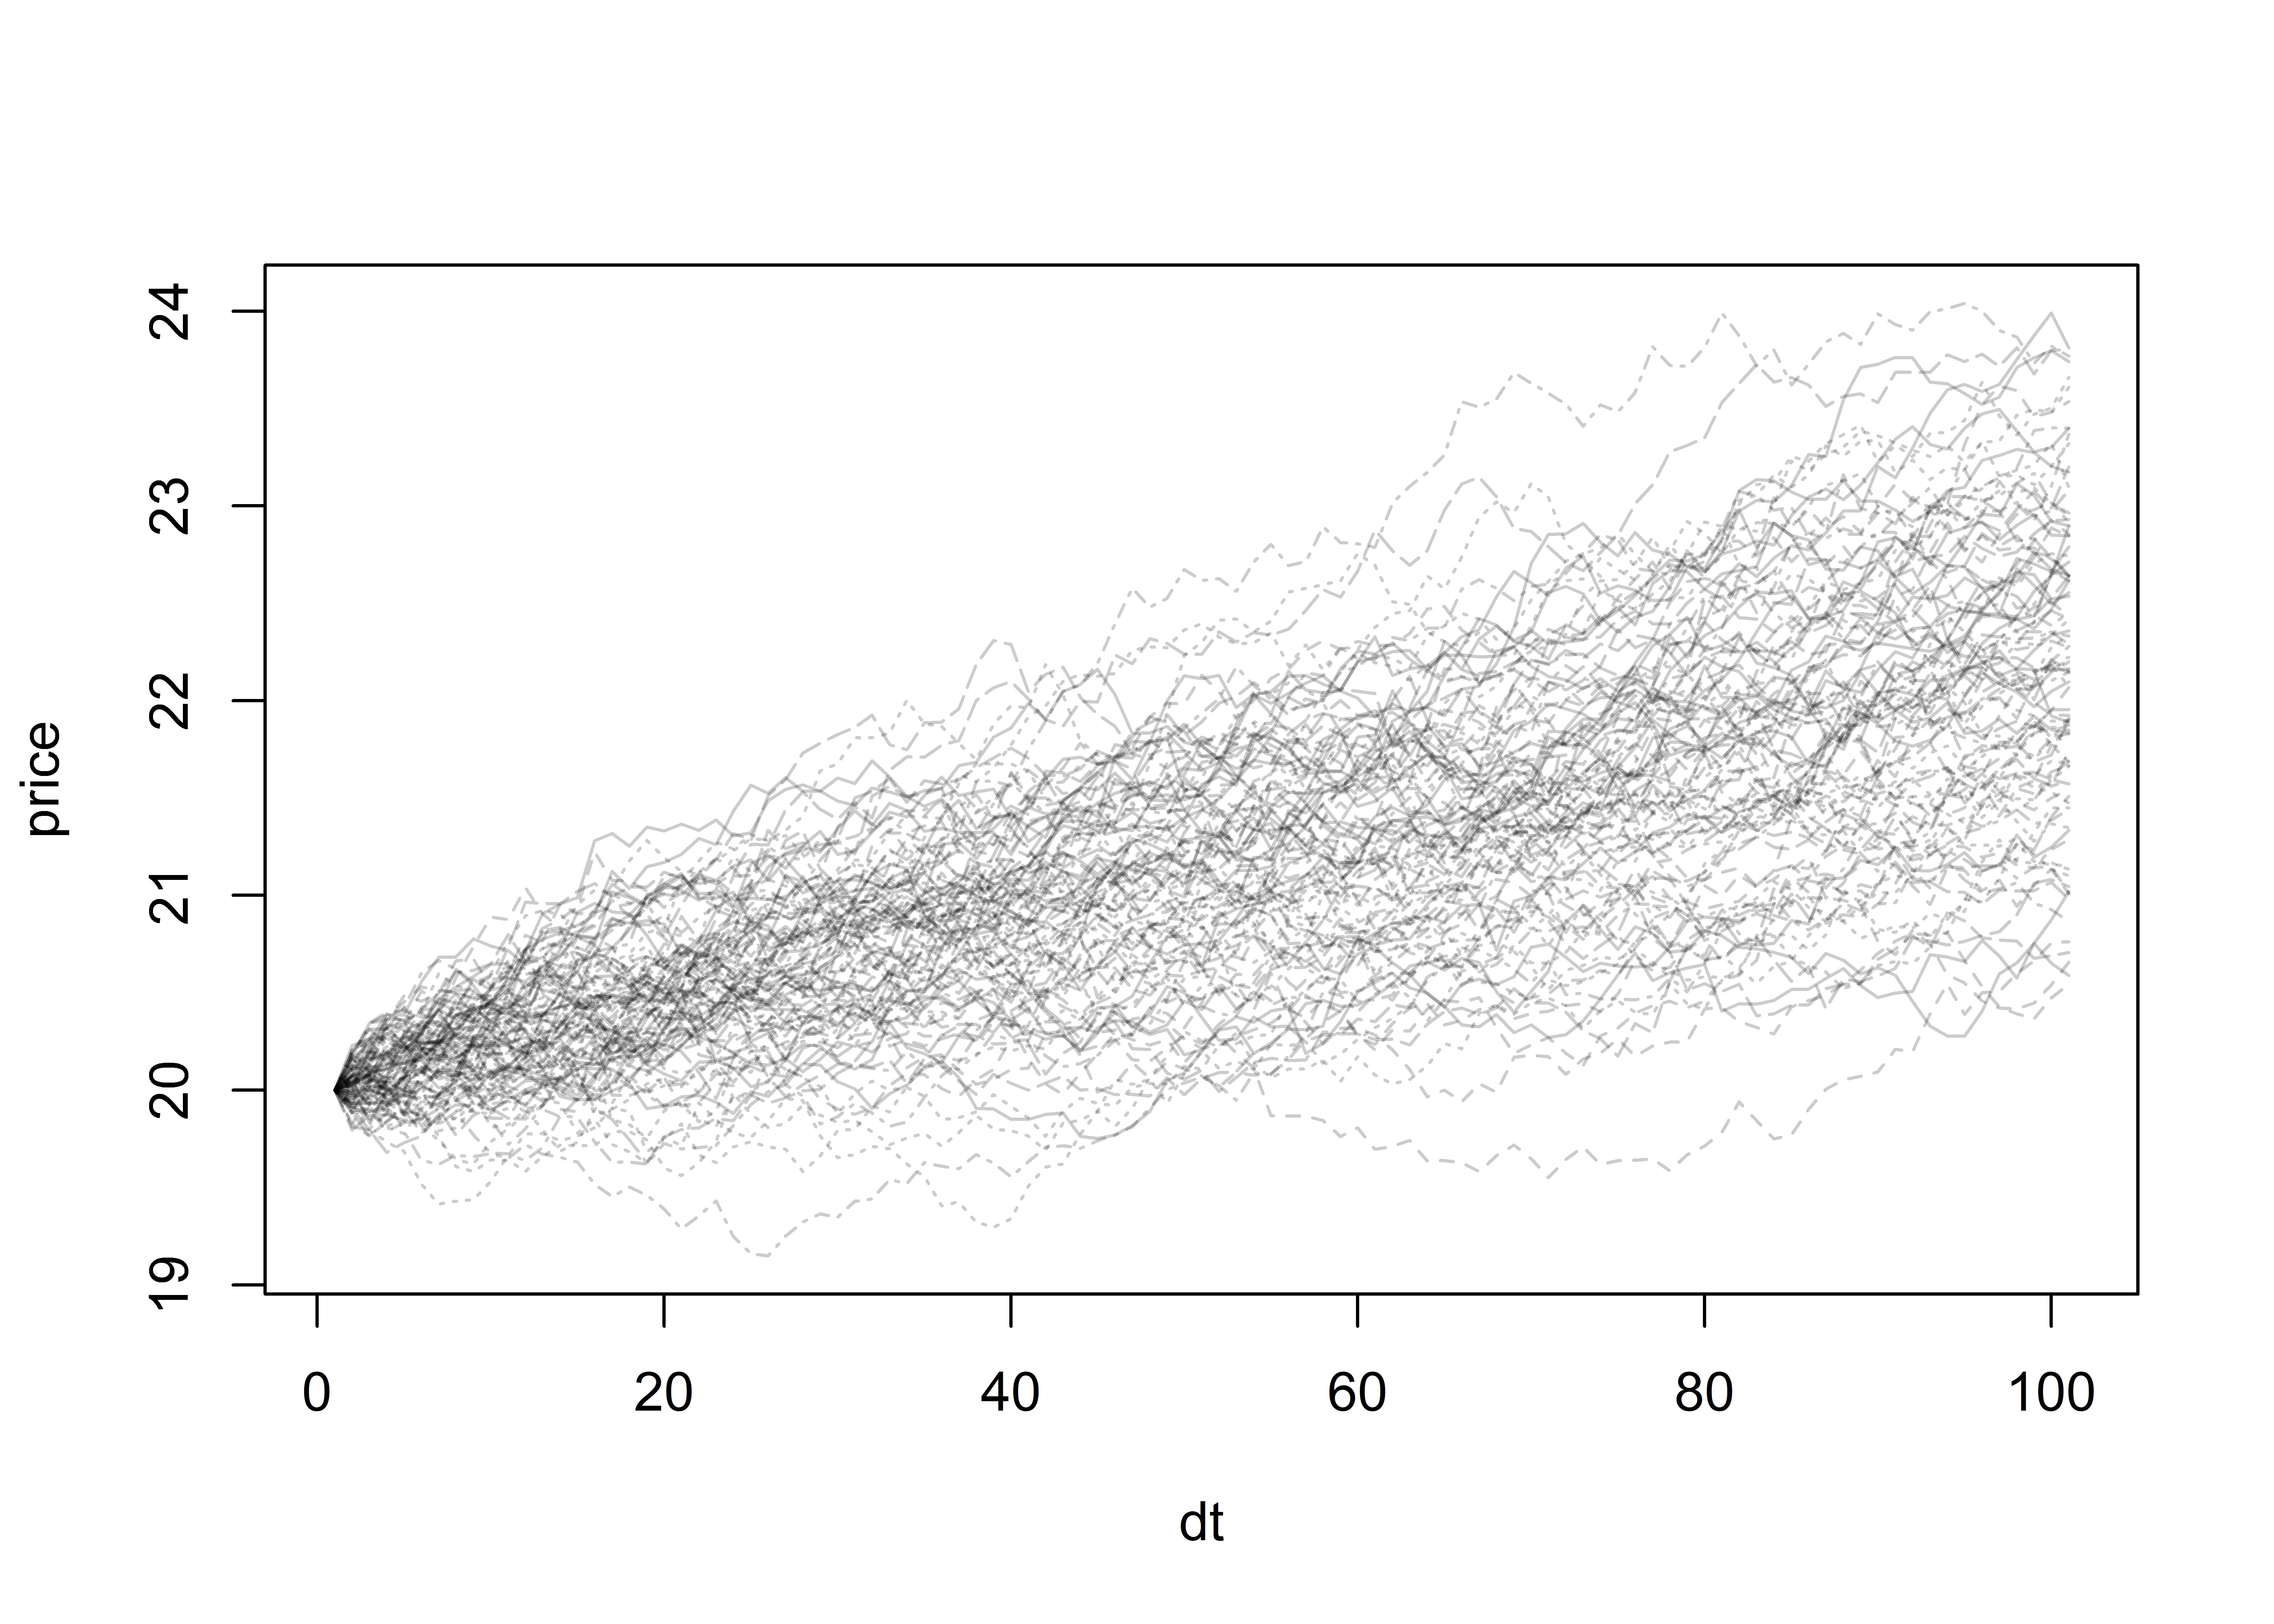
\includegraphics[scale = 0.5]{mc_trajectories.jpeg}
	\caption{Monte Carlo Price Trajectories} \label{img:mc_trajectories}
\end{figure}

From the result shown in Figure \ref{img:mc_trajectories}, we see an collectively upward movement for prices. This corresponds to our setup of a positive drift coefficient of $0.05$.

However, the above code is not computationally efficient. R is relatively slow in running for-loops, and we can speed up the process by using matrix method.

Recall Equation \ref{eq:BS_log_explicit}, where we have the explicit form of $\log(S_t)$. Using similar discretisation method, we can use standard normal random variable $Z$ to substitute $W_t$ to form a recursive equation, such that:

\begin{align*}
\log(S_i) = \log(S_{i-1}) + (\mu - \frac{\sigma^2}{2})\Delta t + \sigma Z_i \sqrt{\Delta t}
\end{align*}

Notice that assume $\Delta t$ is fixed, the part $\log(\Delta S)_i\coloneqq(\mu - \frac{\sigma^2}{2})\Delta t + \sigma Z_i \sqrt{\Delta t}$ is time independent. Therefore:

\begin{align}
\log(S_{i+k}) &= \log(S_{i-1}) + \sum_{j=i}^{k}{\left[(\mu - \frac{\sigma^2}{2})\Delta t + \sigma Z_i \sqrt{\Delta t}\right]} \\
&= \log(S_{i-1}) + \sum_{j=i}^{k}{\log(\Delta S_i)} \label{eq:mc_matrix}
\end{align}

For $i,k\in\mathbb{N}$ and $i+k\leq m$.

This allows us to reduce the two layers of for-loops into matrix operations.

\begin{Rminted}
mc.mat <- function() {
    Z <<- matrix(rnorm(n * m), ncol = n)
    logdS <<- (mu - sigma^2 / 2) * dt + sigma * Z * sqrt(dt)
    logS <<- log(S0) + apply(logdS, 2, cumsum)
    S <<- exp(logS)
    S <<- rbind(S0, S) # Add back the missing row of starting point S0
}
\end{Rminted}

Here, we first define \mintinline{R}|Z| to be a matrix that constains all standard normal random variables required for a total of $n\times m$ number of steps. Then we define \mintinline{R}|logdS| as the matrix of all increments. Based on Equation \ref{eq:mc_matrix}, by using $\log(S_0)$ as the starting point and use cumulative sum \mintinline{R}|cumsum| function to add increament $\log(\Delta S)$ along steps of each trajectory, we will obtain the movement of prices in time. By some further post process shown above, we will get the same result as using the for-loops.

To test the difference in computing speed between the two methods, we will test the average running time using the R package \mintinline{R}|microbenchmark|. The device configuration which the test runs on can be find in Section \ref{sec:machine_env}.

The \mintinline{R}|microbenchmark| function runs individual functions for 100 times and records the summary statistics of the running times, as shown below:

\begin{Rminted}
microbenchmark::microbenchmark(
    mc.for(),
    mc.mat()
)

>     Unit: microseconds
>     expr     min      lq      mean   median      uq     max neval
> mc.for() 18327.2 19872.8 26257.504 25396.45 27853.6 60920.1   100
> mc.mat()   831.8   964.9  1200.425  1039.30  1094.5  8045.3   100
\end{Rminted}

From the result we see that \mintinline{R}|mc.mat| is substantially faster than \mintinline{R}|mc.for|. We shoud thus prefer the former to obtain better estimation efficiency.

The matrix method can also be implemented via the form shown in Equation \ref{eq:mc_explicit} using cumulative product \mintinline{R}|cumprod| function. However, the running time for single multiplication is slightly longer than addition. One may decide to use either methods considering redability and efficiency.

The full look of the \mintinline{R}|mc.engine| is shown below:

\begin{Rminted}
mc.engine <- function(type, K, t, S0, r, q, sigma, n, steps) {

    dt <- t / steps

    # Generate n random samples from N(0,1)
    Z <- matrix(rnorm(n * steps), ncol = n)

    # Get logarithm of price change per step
    increment <- (r - q - sigma^2 / 2) * dt + sigma * sqrt(dt) * Z

    # Use vectorised MC method to compute logarithm of S(t) at each time step
    logS <- log(S0) + apply(increment, 2, cumsum)
    S <- exp(logS) # Obtain the simulated stock price by taking exponential
    S <- S * exp(-q * t) # Adjust the asset price for dividends
    S <- rbind(S0, S) # Add column of current price
    S
}
\end{Rminted}

Notice that the argument specifying the number of time steps to simulate per trajectory, $m$, is now specified under the name \mintinline{R}|steps|.

Here, the drift coefficient is decomposed to (fixed) annual interest rate $r$ and (fixed) annual dividend yield rate $q$ according to Equation \ref{eq:mc_explicit_rq}. The number of time steps $m$ is directly named as \mintinline{R}|steps|.

Adapting this formulation, \mintinline{R}|rmcop| has a function named \mintinline{R}|mc.engine|, which takes the mentioned input arguments and returns a $(m+1)\times n$ matrix recording all generated trajectories. The rest of the functions described in the following subsections takes \mintinline{R}|mc.engine| as an internal component and use the returned matrix to perform further calculations of option payoff.

Using R package \mintinline{R}|profvis|, we can profile the run-time of the function \mintinline{R}|price.option| under a reasonably time-consuming Monte Carlo setup. Here we will simulate 10000 trajectories, each with 1000 time steps. The result trajectory matrix will contain $10000\times1000=10000000$ simulated prices. The code for benchmarking is shown below, and the output is presented in Figure \ref{img:mc_profile}.

\begin{Rminted}
# Creating option and environment objects
op <- option("european", "vanilla", "call", 20, 0.75)
op.env <- option.env(S = 20, r = 0.03, q = 0.01, sigma = 0.05)

# Profiling
profvis::profvis(
    price.option(op, op.env, n = 10000, steps = 1000, all = FALSE, plot = FALSE)
)
\end{Rminted}

\begin{figure}[H]
	\centering
	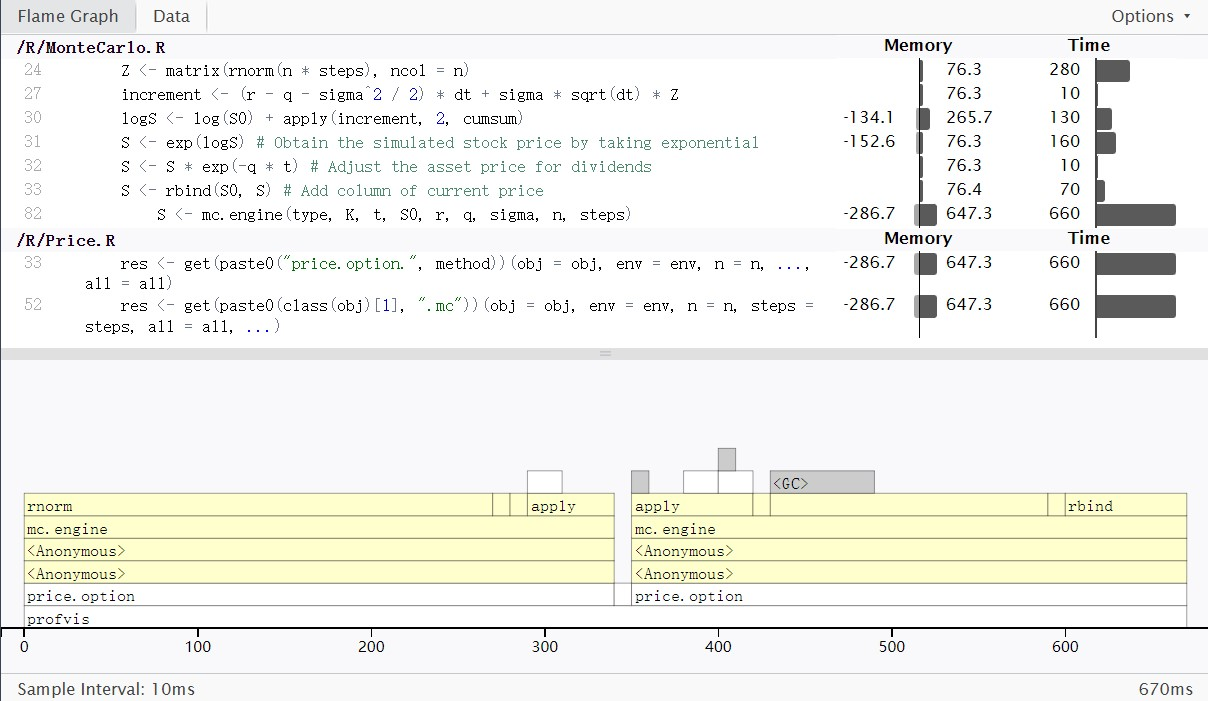
\includegraphics[scale = 0.45]{mc_profile.jpeg}
	\caption{Profiling output of Monte Carlo pricing function} \label{img:mc_profile}
\end{figure}

The named strips in Figure \ref{img:mc_profile}, represents different components that are triggered when running \mintinline{R}|price.option|. Each function represented by the corresponding strip is the internal component of the one below it. Here, we see \mintinline{R}|mc.engine| is the most (and only) time consuming component of the pricing function. This means our prior adjustment of replacing for-loops with more efficient matrix operation is essensial for reducing the computing cost of the whole pricing procedure.

An additional component is added to calculate the Standard Error of estimation. The formula used is shown by Equation \ref{eq:mc_SE}:

\begin{Rminted}
mc.SE <- function(C_i, C.mean, n) {
    s_c <- sqrt(sum(C_i - C.mean)^2 / (n - 1))
    SE <- s_c / sqrt(n)
    SE
}
\end{Rminted}

The resulting standard error can be used to construct confidence intervals of the estimate of the option price.

One should be aware that Monte Carlo option pricing for American options is beyond the scope of this report. In the pricing functions below, we will only consider the pricing of European options.

\subsection{vanilla.mc}

The pricing of Vanilla options is examplified in Equation \ref{eq:discount_vanilla_payoff}. To obtain the simulated $S_T$'s, one shall simply take the last row of the matrix output from the \mintinline{R}|mc.engine| and directly translate the formula to R code:

\begin{Rminted}
if (type == "call") {
    C <- exp(-r * t) * pmax(S[steps + 1, ] - K, 0)
} else if (type == "put") {
    C <- exp(-r * t) * pmax(K - S[steps + 1, ], 0)
}
\end{Rminted}

Where the resulting discounted payoffs for each trajectory is stored in the vector \mintinline{R}|C|.

Notice that for a path-independent option such as an Vanilla option, we are only considering the option price at expiration. Thus, it is reasonable to take \mintinline{R}|step = 1| to reduce computational cost.

\subsection{asian.mc}

Exotic options such as Asian options and those included below are path-dependent. This implies capturing the price movements throughout time $t\in[0,T]$ is necessary.

Recall from Section \ref{sec:Literature Review}, an Asian option's payoff is revelent to the underlying asset's average price through $t=[0,T]$. Thus, we will first compute and store the average prices of each trajectory.

\begin{Rminted}
S.mean <- apply(S, 2, mean)
\end{Rminted}

The \mintinline{R}|apply| function with the second argument set to \mintinline{R}|2| allows us to apply the operation \mintinline{R}|mean| on each column of \mintinline{R}|S|, thus giving us the average price of each trajectory.

After obtaining the average, we will directly implement the payoff functions showed in List \ref{lst:exotic_options} in R as shown below:

\begin{Rminted}
if (is.avg_price) { # Compute payoff for average price Asian option
    if (type == "call") {
        C <- exp(-r * t) * pmax(S.mean - K, 0)
    } else if (type == "put") {
        C <- exp(-r * t) * pmax(K - S.mean, 0)
    }
} else { # Compute payoff for average strike Asian option
    if (type == "call") {
        C <- exp(-r * t) * pmax(S[steps + 1, ] - S.mean, 0)
    } else if (type == "put") {
        C <- exp(-r * t) * pmax(S.mean - S[steps + 1, ], 0)
    }
}
\end{Rminted}

Notice that for path dependent cases, using large enough number of steps for each simulation to better resemble the real-world scenario is necessary to obtain an accurate approximation.

\subsection{barrier.mc}

As we see from List \ref{lst:exotic_options}, a barrier option is ``switched on and off'' depending on whether the price movements crossed some pre-defined price barrier. To record this pre-specified quantity, we require user to include a property named \mintinline{R}|barrier| when they define their option object. We also require users to specify a boolean argument named \mintinline{R}|is.knockout| to classify whether the barrier option is ``knock-in'' or ``knock-out''. This is demonstrated by the below example:

\begin{Rminted}
option(style = "european", option = "barrier", type = "call", K = 20, t = 1, barrier = 21, is.knockout = TRUE)
\end{Rminted}

Here, besides from the regular parameters to see in any option, the user defined the barrier price to be $21$ and the option to be a ``knock-out'' barrier option, meaning that the option payoff will be zero if the price movement crossed the value $21$.

To determine whether a price trajectory crossed certain level, we can record the minimum and maximum through the trajectory and see if the barrier value lies between two extremas. If so, because the price trajectory is continuous, we know that the trajectory must have crossed the barrier at least once through the option's life time.

We will use similar \mintinline{R}|apply| method as mentioned in the previous section. Only now, we are computing the minimums and maximums of the trajectories. We then use a boolean vector \mintinline{R}|is.cross| to determine whether the barrier is bounded by the extremas.

\begin{Rminted}
S.min <- apply(S, 2, min)
S.max <- apply(S, 2, max)
is.cross <- (S.min < barrier & S.max > barrier)
\end{Rminted}

We know that a barrier option would behave exactly the same as a vanilla option if ignoring the ``knock-in/out'' effect, so we will first calculate its discounted payoff with the exact same methods in the above vanilla option pricing section.

\begin{Rminted}
if (type == "call") {
    C <- exp(-r * t) * pmax(S[steps + 1, ] - K, 0)
} else if (type == "put") {
    C <- exp(-r * t) * pmax(K - S[steps + 1, ], 0)
}
\end{Rminted}

Then, we take into account of the special effect and decide whether to zero the option payoff.

\begin{Rminted}
if (is.knockout) { # Case for knock-out barrier option
    C <- ifelse(is.cross, 0, C)
} else { # Case for knock-in barrier option
    C <- ifelse(is.cross, C, 0)
}
\end{Rminted}

The function \mintinline{R}|ifelse(condition, A, B)| is simply a quick command for the regular if-else statement. It execute expression \mintinline{R}|A| if \mintinline{R}|condition| is evaluated to \mintinline{R}|TRUE|, and execute \mintinline{R}|B| otherwise.

\subsection{binary.mc}

As we see from List \ref{lst:exotic_options}, a binary option, unlike other options discussed in the report, has a fixed payoff. To record this characteristic, we require user to passin a value for argument \mintinline{R}|payout| when defining a binary option object, as shown in the example below:

\begin{Rminted}
option(style = "european", option = "binary", type = "call", K = 20, t = 1, payout = 5)
\end{Rminted}

For each trajectory, to decide whether the payoff should be zero or the specified value, we simply compare the simulated price at maturity $S_T$ with the strike price $K$. This characteristic also makes a regular binary option path-independent.

Since the payoff is fixed by the variable \mintinline{R}|payout|, for simplicity, we can first set the discounted payoff of every trajectory to be equal, and reduced the ``turned-off'' cases to zero afterwards:

\begin{Rminted}
# Genearte a column vector with the same discounted payoff
C <- matrix(exp(-r * t) * payout, nrow = n, ncol = 1)

# Based on the specific type of the option, reduced corresponding rows to zero based on the payoff formula for binary option
if (type == "call") {
    C <- ifelse(S[steps + 1, ] > K, C, 0)
} else if (type == "put") {
    C <- ifelse(S[steps + 1, ] < K, C, 0)
}
\end{Rminted}

\subsection{lookback.mc}

A lookback option is another case of a path-dependent option. As we see from List \ref{lst:exotic_options}, a fixed strike lookback's payoff is determined by comparing the price extramas and the strike price throughout the life time, and a floating strike lookback's payoff is by comparing the price extramas and the price at maturity. This makes the lookback option being obviously path-dependent.

To determine whether the pre-specified lookback option is fixed or floating, we require the user to passin a value for the boolean variable \mintinline{R}|is.fixed|, which indicates the option is ``fixed strike'' if evaluated to \mintinline{R}|TRUE|, and being ``floating strike'' otherwise. This is shown in the codes below:

\begin{Rminted}
option(style = "european", option = "lookback", type = "call", K = 20, t = 1, is.fixed = TRUE)
\end{Rminted}

To allow us to calculate the payoff for each trajectory, we will first store the required value of minimum and maximum prices for each simulation, this could be done using the similar \mintinline{R}|apply| method as demonstrated above:

\begin{Rminted}
S.min <- apply(S, 2, min)
S.max <- apply(S, 2, max)
\end{Rminted}

And the vector containing the simulated prices at maturity can be done with the same \mintinline{R}|S[steps + 1, ]| command.

After obtaining these elements, based on the classification of lookback options, there are 4 scenarios for the payoff to be calculated. By directly implement the formulas as displayed in \ref{lst:exotic_options}, we will obtain the vector \mintinline{R}|C| of discounted payoffs.

\begin{Rminted}
if (type == "call") {
    if (is.fixed) { # Fixed strike
        C <- exp(-r * t) * pmax(S.max - K, 0)
    } else { # Float strike
        C <- exp(-r * t) * (S[steps + 1, ] - S.min)
    }
} else if (type == "put") {
    if (is.fixed) { # Fixed strike
        C <- exp(-r * t) * pmax(K - S.min, 0)
    } else { # Float strike
        C <- exp(-r * t) * (S.max - S[steps + 1, ])
    }
}
\end{Rminted}

\newpage